\chapter{Ergebnisse} \label{sec:results}

Das Kapitel stellt die Ergebnisse der Tests der verschiedenen Modelle dar. Außerdem 
wird eine Übersicht über die benötigte Trainingszeit für die Modelle gegeben. 

\section{Benötigte Trainingszeit}

\begin{itemize}
    \item Eine Epoche des Pre-Trainings auf dem Combined-Straßendatensatz dauert zwischen 40 und 50 Minuten. 
    \item Eine Epoche des Trainings auf dem BikeSat-Datensatz dauert zwischen 10 und 17 Minuten. 
    \item Die Netze konvergieren nach circa 33-57 Epochen auf beiden Datensätzen. 
    \item Das Training wird immer vorzeitig vor dem Ablaufen der 100 Epochen beendet.
    \item Der zeitliche Mehraufwand durch die Bild-Augmentierung während des Trainings (vgl. \autoref{sec:pre-processing}) 
    liegt im Schnitt bei 3 min 30s pro Epoche für beide Augmentierungsmethoden (Basic-Augmentation und Color-Augmentation).  
\end{itemize}

\section{Pre-Training-Ergebnisse zur Straßenerkennung}

\begin{table}[ht]
	\centering
	\begin{tabular}{l|c|c}
		Modell & \ac{IoU} & \ac{BIoU} \\
		\midrule
        BUNet2 & 57,13 & 76,71 \\ 
        BUNet15 & 60,75 & 80,80 \\ 
        VBUNet & \textbf{64,26} & \textbf{85,64} \\ 
        RBUNet & 61,45 & 83,86 \\ 
        DBUNet & 62,56 & 84,46 \\ 
        
	\end{tabular}
	\caption{Ergebnisse des Pre-Trainings der Modelle auf der Testpartition des Combined-Datensatzes in Prozent.}
	\label{tab:results-roads}
\end{table}

\begin{figure}
	\centering
	\begin{minipage}{.41\textwidth}
		\centering
		\includegraphics[width=1.\linewidth]{Bilder/Samples-Combined/bunet2.png}
	\end{minipage}
	\begin{minipage}{.41\textwidth}
		\centering
		\includegraphics[width=1.\linewidth]{Bilder/Samples-Combined/vbunet.png}
	\end{minipage}

	\caption{Beispiel-Predictions des $BUNet2$ (links) und $VBUNet$ (rechts) auf dem Combined-Datensatz.}
	\label{fig:combined-samples-bune2-vbunet}
\end{figure}

\autoref{tab:results-roads} zeigt die Test-Ergebnisse der Modelle nach Training auf dem Combined-Datensatz 
(vgl. \autoref{sec:pre-training-roads}) in Prozent. Pro Spalte ist das höchste Ergebnis hervorgehoben. 
\ac{BUNet2} und \ac{BUNet15} sind von Grund auf trainiert, während \ac{VBUNet}, \ac{RBUNet} und \ac{DBUNet} einen auf 
ImageNet vortrainierten Encoder aufweisen. Die \ac{BIoU} verwendet wie bei der Radwegerkennung und wie in \autoref{sec:eval:biou} 
festgelegt eine Puffergröße von 15 Pixeln. \\ 
BUNet2 schneidet am schlechtesten ab, während VBUNet die höchsten Werte für IoU und BIoU aufweist. 
Generell sind alle Netze mit vortrainiertem Backbone besser, als die nicht vortrainierten Netze 
der BUNet-Archtiektur. 

\autoref{fig:combined-samples-bune2-vbunet} zeigt ausgewählte Beispielpredictions des \ac{BUNet2} (links) und 
des \ac{VBUNet} (rechts).\footnote{Weitere Beispiele anderer Netze in \autoref{sec:pred-combined}.} \\
Es ist zu erkennen, dass beide Netze die Straßen größtenteils richtig erkennen. 
BUNet2 zeichnet dabei etwas unschärfere Linien, wie aus Bild zwei (gepunktet) und aus Bild vier 
(keine schwarze Linie zwischen der breiten Straße) hervorgeht. Im dritten Bild von unten 
auf der rechten Seite ist rechts oben ein Gebäude zu erkennen, welches über den Highway geht. 
In der Maske ist dort an der Stelle des Gebäudes die Straße weiter annotiert. 
In der Prediction von VBUNet ist dieser Teil jedoch ausgespart.  

\section{Ergebnisse der Radwegerkennung}

\begin{table}[ht]
	\centering
	\begin{tabular}{l|cc|cc|cc|cc}
		& \multicolumn{4}{c|}{Basic Augmentation} & \multicolumn{4}{c}{Color Augmentation} \\
        & \multicolumn{2}{c|}{BikeSat} & \multicolumn{2}{c|}{Karlsruhe} & \multicolumn{2}{c|}{BikeSat} & \multicolumn{2}{c}{Karlsruhe} \\
		Modell & \ac{IoU} & \ac{BIoU} & \ac{IoU} & \ac{BIoU} & \ac{IoU} & \ac{BIoU} & \ac{IoU} & \ac{BIoU} \\
		\toprule
        BUNet2$^*$ & 23,54 & 47,71 & 01,30 & 34,80 &  27,47 & 55,19 & 12,69 & 47,53 \\
        BUNet2$^l$ & 24,48 & 51,77 & 02,19 & 12,11 &  28,06 & 57,21 & 08,54 & 39,19 \\
        BUNet2$^r$ & 25,35 & 51,27 & 09,36 & 47,57 &  25,95 & 53,73 & 04,56 & 25,97 \\
		\midrule

        BUNet15$^*$ & 27,93 & 56,55 & \textbf{21,52} & \textbf{59,25} &  30,80 & 59,99 & 06,84 & 33,23 \\
        BUNet15$^l$ & 28,14 & 57,14 & 16,47 & 54,17 &  30,98 & 60,50 & 07,47 & 30,20 \\
        BUNet15$^r$ & 28,22 & 57,26 & 10,17 & 53,81 &  29,95 & 59,46 & 08,23 & 26,82 \\
		\midrule

        VBUNet$^*$ & 30,45 & 61,48 & 09,69 & 37,84 &  \textbf{31,71} & \textbf{61,32} & 09,29 & 31,15 \\
        VBUNet$^l$ & \underline{\textbf{32,24}} & \textbf{62,93} & 12,85 & 54,91 &  21,91 & 45,88 & 03,19 & 23,25 \\
        VBUNet$^r$ & \textbf{31,84} & 61,51 & 17,53 & \textbf{61,51} &  25,65 & 51,82 & 10,74 & 32,31 \\
		\midrule

        RBUNet$^*$ & 29,11 & 60,53 & 11,74 & 32,80 &  \underline{\textbf{33,54}} & \underline{\textbf{65,02}} & \textbf{23,24} & \textbf{65,71} \\
        RBUNet$^l$ & 30,98 & 60,51 & \underline{\textbf{24,67}} & \underline{\textbf{65,27}} &  29,32 & 59,83 & 09,67 & 53,08 \\
        RBUNet$^r$ & 31,31 & \underline{\textbf{63,55}} & \textbf{18,21} & 55,53 &  29,42 & 59,58 & \underline{\textbf{34,66}} & \underline{\textbf{68,26}} \\
		\midrule

        DBUNet$^*$ & 30,76 & 61,78 & 07,14 & 45,97 &  \textbf{32,24} & \textbf{64,77} & 14,64 & 50,02 \\
        DBUNet$^l$ & 31,55 & 62,38 & 17,47 & 55,20 &  29,64 & 60,47 & 14,83 & 51,19 \\
        DBUNet$^r$ & \textbf{32,12} & \textbf{62,99} & 14,03 & 51,73 &  30,30 & 61,24 & 17,43 & \textbf{62,28} \\
        
		\bottomrule
		\multicolumn{1}{r|}{$\bar{x}$} & 29,20 & 58,62 & 12,96 & 48,16 & 29,13 & 58,40 & 12,40 & 42,68 \\
		\midrule
		\multicolumn{1}{r|}{s} & 02,86 & 04,91 & 06,61 & 13,76 & 02,96 & 05,00 & 08,03 & 15,20 \\


	\end{tabular}
	\caption{Ergebnisse der Modelle auf der Testpartition des BikeSat-Datensatzes und dem Karlsruhe-Datensatz
	für beide Augmentierungsmethoden. 
    In Prozent.}
	\label{tab:results}
\end{table}

\autoref{tab:results} zeigt die Test-Ergebnisse der Modelle nach Training (s. \autoref{sec:training} für Details) auf dem BikeSat-Datensatz 
(s. \autoref{sec:bike-data}) für jede Augmentierungsmethode (Basic- u. Color-Augmentation) während des Trainings in Prozent. 
Zusätzlich zeigt die Tabelle die Test-Ergebnisse auf allen 196 $512{\times}512$-Ausschnitten 
des Karlsruhe-Datensatz (s. \autoref{sec:karlsruhe}) in Prozent. Der Karlsruhe-Datensatz in dieser Tabelle
enthält auch Ausschnitte, die \textit{keine} Radwege enthalten. \\ 
Pro Spalte sind die höchsten drei Ergebnisse hervorgehoben und das höchste unterstrichen. 
Außerdem sind pro Spalte das arithmetische Mittel $\bar{x}$ und die Standardabweichung s angegeben. 
Die \ac{BIoU} hat eine Puffergröße von 15 Pixeln, wie in \autoref{sec:eval:biou} festgelegt.
\begin{enumerate}
	\item Die Modelle performen statistisch signifikant\footnote{
		$p = 2,143\cdot 10^{-8}$ für die IoU und $p = 0,00639$ für die BIoU für Basic-Aug. und 
		$p = 2,937\cdot 10^{-7}$ für die IoU und $p = 7,06 \cdot 10^{-4}$ für die BIoU für Color-Aug.
		des einseitigen Zweistichproben-Welch-Tests zwischen BikeSat und Karlsruhe. 
	} stärker auf der Testpartition des BikeSat-Datensatzes, mit ein paar Ausnahmen, wie z.B. dem RBUNet$^r$ auf Color-Augmentation trainiert, 
	als auf dem Karlsruhe-Datensatz. 
	\item Die Ergebnisse auf dem BikeSat-Datensatz sind deutlich stabiler und zwischen den Netzen ähnlicher, weisen also eine signifikant \footnote{
		$p = 0,0035$ für die IoU und $p = 4,38\cdot 10^{-4}$ für die BIoU für Basic-Aug. und 
		$p = 6,21\cdot 10^{-4}$ für die IoU und $p = 1,72 \cdot 10^{-4}$ für die BIoU für Color-Aug.
		des F-Tests zwischen BikeSat und Karlsruhe. 
	} geringere Streuung auf, als auf dem Karlsruhe-Datensatz.
	\item Die \ac{IoU} und \ac{BIoU} unterscheiden sich teilweise stark innerhalb eines Modells auf dem Karlsruhe Datensatz (s. z.B. BUNet2$^*$ auf Basic-Augmentation).
	\item Die Netze, die mit Color-Augmentation trainiert sind, erzielen insgesamt höhere Spitzenwerte auf beiden Datensätzen. 
	\item Bei den Backbone-Netzen ist im Schnitt keine Verbesserung von Basic-Augmentation zu Color-Augmentation zu beobachten. 
	\item Für die Netze der BUNet-Architektur führte die Color-Augmentation allgemein zu einer besseren Performance auf dem BikeSat-Datensatz, nicht jedoch auf dem Karlsruhe-Datensatz.
	\item Für Basic-Augmentation performen die vortrainierten Netze generell besser, als die nicht-vortrainierten Gegenstücke. 
	Für Color-Augmentation ist es, zumindest für die Backbone-Netze, genau umgekehrt. 
	\item RBUNet$^r$ liefert als einzige Architektur über beide Augmentierungsmethoden und alle Maßzahlen solide Ergebnisse. 
	Für die Color-Augmentation liefert RBUNet$^*$ konsequent sehr gute Ergebnisse, während für Basic-Augmentation RBUNet$^l$ konsequent sehr gute Ergebnisse liefert.
\end{enumerate}


\begin{table}[ht]
	\centering
	\begin{tabular}{l|cc|cc|cc}
        & \multicolumn{2}{c|}{\textcolor{gray}{BikeSat}} & \multicolumn{2}{c|}{\textcolor{gray}{Karlsruhe}} & \multicolumn{2}{c}{Wolfsburg} \\
		Modell & \textcolor{gray}{\ac{IoU}} & \textcolor{gray}{\ac{BIoU}} & \textcolor{gray}{\ac{IoU}} & \textcolor{gray}{\ac{BIoU}} & \ac{IoU} & \ac{BIoU} \\
		\toprule
        BUNet2$^*$ & \textcolor{gray}{27,47} & \textcolor{gray}{55,19} & \textcolor{gray}{12,69} & \textcolor{gray}{47,53} &  28,44 & 57,30 \\
        BUNet2$^l$ & \textcolor{gray}{28,06} & \textcolor{gray}{57,21} & \textcolor{gray}{08,54} & \textcolor{gray}{39,19} &  29,92 & 59,64 \\
        BUNet2$^r$ & \textcolor{gray}{25,95} & \textcolor{gray}{53,73} & \textcolor{gray}{04,56} & \textcolor{gray}{25,97} &  28,62 & 57,98 \\
		\midrule

        BUNet15$^*$ & \textcolor{gray}{30,80} & \textcolor{gray}{59,99} & \textcolor{gray}{06,84} & \textcolor{gray}{33,23} &  30,68 & 61,86 \\
        BUNet15$^l$ & \textcolor{gray}{30,98} & \textcolor{gray}{60,50} & \textcolor{gray}{07,47} & \textcolor{gray}{30,20} &  31,31 & 61,71 \\
        BUNet15$^r$ & \textcolor{gray}{29,95} & \textcolor{gray}{59,46} & \textcolor{gray}{08,23} & \textcolor{gray}{26,82} &  30,99 & 60,84 \\
		\midrule

        VBUNet$^*$ & \textcolor{gray}{\textbf{31,71}} & \textcolor{gray}{\textbf{61,32}} & \textcolor{gray}{09,29} & \textcolor{gray}{31,15} &  \textbf{32,90} & \textbf{66,08} \\
        VBUNet$^l$ & \textcolor{gray}{21,91} & \textcolor{gray}{45,88} & \textcolor{gray}{03,19} & \textcolor{gray}{23,25} &  22,79 & 50,18 \\
        VBUNet$^r$ & \textcolor{gray}{25,65} & \textcolor{gray}{51,82} & \textcolor{gray}{10,74} & \textcolor{gray}{32,31} &  27,53 & 56,97 \\
		\midrule

        RBUNet$^*$ & \textcolor{gray}{\underline{\textbf{33,54}}} & \textcolor{gray}{\underline{\textbf{65,02}}} & \textcolor{gray}{\textbf{23,24}} & \textcolor{gray}{\textbf{65,71}} &  \underline{\textbf{34,42}} & \textbf{67,74} \\
        RBUNet$^l$ & \textcolor{gray}{29,32} & \textcolor{gray}{59,83} & \textcolor{gray}{09,67} & \textcolor{gray}{53,08} &  30,80 & 63,30 \\
        RBUNet$^r$ & \textcolor{gray}{29,42} & \textcolor{gray}{59,58} & \textcolor{gray}{\underline{\textbf{34,66}}} & \textcolor{gray}{\underline{\textbf{68,26}}} &  31,17 & 63,47 \\
		\midrule

        DBUNet$^*$ & \textcolor{gray}{\textbf{32,24}} & \textcolor{gray}{\textbf{64,77}} & \textcolor{gray}{14,64} & \textcolor{gray}{50,02} &  \textbf{33,70} & \underline{\textbf{68,48}} \\
        DBUNet$^l$ & \textcolor{gray}{29,64} & \textcolor{gray}{60,47} & \textcolor{gray}{14,83} & \textcolor{gray}{51,19} &  31,02 & 63,21 \\
        DBUNet$^r$ & \textcolor{gray}{30,30} & \textcolor{gray}{61,24} & \textcolor{gray}{\textbf{17,43}} & \textcolor{gray}{\textbf{62,28}} &  31,48 & 64,48 \\

		\bottomrule
		\multicolumn{1}{r|}{$\bar{x}$} & 29,13 & 58,40 & 12,40 & 42,68 & 30,38 & 61,55 \\
		\midrule
		\multicolumn{1}{r|}{s} & 02,96 & 05,00 & 08,03 & 15,20 & 02,81 & 04,71 \\
		
		
        
	\end{tabular}
	\caption{Ergebnisse der Modelle auf dem Wolfsburg-Datensatz mit farbverändernden Augmentierungen (Color-Aug.). In Prozent.
	(Die Ergebnisse von BikeSat und Karlsruhe entsprechen \autoref{tab:results} und sind zur einfacheren Vergleichbarkeit erneut aufgeführt.)}
	\label{tab:results-wolfsburg}
\end{table}

\autoref{tab:results-wolfsburg} ergänzt \autoref{tab:results} um die Ergebnisse auf dem Wolfsburg-Datensatz für 
Training mit Color-Augmentation. Zur besseren Übersichtlichkeit sind die Ergebnisse für Basic-Aug. hier ausgespart, 
da diese weniger interessant sind. 
\begin{enumerate}
	\item Es fällt auf, dass sowohl die \ac{IoU} als auch die \ac{BIoU} für alle Modelle
	auf dem Wolfsburg-Datensatz besser ist, als auf der Testpartition des BikeSat-Datensatzes 
	(mit Ausnahme der IoU von $BUNet15^*$).  \\
	Selbiges gilt für den Vergleich von Wolfsburg mit Karlsruhe, bis auf die Modelle VBUNet$^l$ und 
	RBUNet$^r$, die auf dem Karlsruhe-Datensatz in IoU sowie BIoU höhere Werte erzielen, als auf dem Wolfsburg-Datensatz. \\
	Statistisch signifikante Unterschiede erzielen die BIoU von BikeSat zur BIoU von Wolfsburg ($p = 0,043$), 
	sowie die IoU und BIoU von Karlsruhe zu Wolfsburg ($p = 1,14 \cdot 10^{-7}$, bzw. $1,36 \cdot 10^{-4}$). 
	Die Differenz von IoU des BikeSat-Datensatzes zur IoU des Wolfsburg-Datensatzes verfehlt die statistische Signifikanz 
	mit $p = 0,122$.\footnote{Alle Tests als einseitige Zweistichproben-Welch-Tests.}  
	\item Über alle Datensätze performt RBUNet$^*$ am besten. Es liefert über alle sechs Maßzahlen Top-3-Ergebnisse wobei es 
	in für drei davon am besten performt. 
	\item Darüber hinaus ist auffällig, wie viel schlechter die vortrainierten Varianten der VBUNet-Architektur performen. 
	Während VBUNet$^*$ auf dem BikeSat- und Wolfsburg-Datensatz solide Ergebnisse liefert, liegen VBUNet$^l$ und VBUNet$^r$ 
	weit unterhalb. Bei der IoU 10 Prozentpunkte, bei der BIoU bis zu 16 Prozentpunkte.
	\item Generell performen die Netze der \ac{BUNet2}-Architektur schlechter als die der \ac{BUNet15}-Architektur.
	\item Interessanterweise performen die vortrainierten Modelle der Backbone-Architekturen auf dem BikeSat- und 
	Wolfsburg-Datensatz konstant schlechter als die nicht vortrainierten. Die rechtsseitig vortrainierten zeigen 
	allerdings bessere Performance auf dem Karlsruhe-Datensatz, als die anderen Modelle der jeweiligen Backbone-Archtiektur.\\
	Für Modelle der BUNet-Architektur sind die Ergebnisse recht ähnlich und es ist keine schlechtere Performance
	zu beobachten. 
\end{enumerate}


\subsection{Beispiel-Predictions ausgewählter Netze} \label{sec:example-preds}

\autoref{fig:bikesat-samples-bunet2-s-vbunet-l} zeigt ausgewählte Beispielpredictions des $BUNet2^*$ (a) und 
des $VBUNet^l$ (b) auf dem BikeSat-Datensatz bei Training mit Basic-Augmentation.\footnote{Weitere Beispiele anderer Netze in \autoref{sec:pred-bikesat}.}
\begin{itemize}
	\item Es fällt auf, dass einige der Predictions sehr akkurat sind und eine hohe Kongruenz zur Maske aufweisen,
	wie zum Beispiel das zweite Bild von oben zeigt. Andere Predictions deuten allerdings nur qualitativ den Radweg an, 
	wie zum Beispiel die gepunktete Prediction aus Bild vier von oben links zeigt.
	\item Es werden Wege, die von der Beschaffenheit Radwege sein könnten als solche erkannt, 
	obwohl es sich um keine handelt, wie links das sechste Bild von oben zeigt. Auch haben beide Netze 
	auf den Bildern zwei und drei von unten auf beiden Straßenseiten Radwege erkannt, obwohl nur auf einer tatsächlich einer ist.
	Bei Bild vier von unten zeigen sich sehr gute Predictions durch beide Netze, da hier korrekterweise nur eine Straßenseite 
	mit Radweg versehen ist. 
	\item Generell geht die quantitativ gemessene bessere Performance von VBUNet$^l$ empirisch aus den Bildern hervor.
\end{itemize}

\autoref{fig:ka-samples-rbunet-l-rbunet-s} zeigt ausgewählte Beispielpredictions des $RBUNet^l$ (a) und 
des $RBUNet^*$ (b) auf dem Karlsruhe-Datensatz bei Training mit Basic-Augmentation.\footnote{Weitere Beispiele anderer Netze in \autoref{sec:pred-karlsruhe}.}
\begin{itemize}
	\item Es ist zu sehen, dass insgesamt die Predictions unschärfer sind im Vergleich zu den Predictions auf dem 
	BikeSat-Datensatz. So gibt es kaum mit den Masken kongruente Bereiche und die Radwege sind oft nur 
	qualitativ durch unterbrochene oder gepunktete Linien angedeutet. 
	\item RBUNet$^*$ kann die ersten sieben Bilder qualitativ recht gut predicten, erkennt aber auf den letzten 
	drei Bildern auch eher Radwege wo keine sind - viele Falsch-Positive also. 
	Das Modell weist eine eher relativ hohe Sensitivität auf. \\
	RBUNet$^l$ hingegen erkennt generell kaum Radwege, aber weist auch keine Falsch-Positiven auf, 
	was kein Radweg ist, wird auch zuverlässig als negativ eingestuft. Dieses Modell hat also eine hohe Spezifität.     
\end{itemize}

\autoref{fig:ka-samples-rbunet-l-rbunet-s-color} zeigt ausgewählte Beispielpredictions des $RBUNet^l$ (a) und 
des $RBUNet^*$ (b) auf dem Karlsruhe-Datensatz bei Training mit Color-Augmentation. \\
 Durch das veränderte Training mit Color-Augmentation hat sich die Art, wie die Modelle predicten, 
	im Gegensatz zu \autoref{fig:ka-samples-rbunet-l-rbunet-s}, geändert. RBUNet$^l$ weist nun ein paar 
	Falsch-Positive aber auch mehr Wahr-Positive auf. RBUNet$^*$ zeichnet dünnere Linien und erzeugt 
	weniger Wahr-Positive, aber auch weniger Falsch-Positive. Generell scheinen die beiden Netze ähnlicher zu predicten. 

\autoref{fig:wolfsburg-samples-rbunet-l-rbunet-s-color} zeigt ausgewählte Beispielpredictions des $RBUNet^l$ (a) und 
des $RBUNet^*$ (b) auf dem Wolfsburg-Datensatz bei Training mit Color-Augmentation. \\
Die Predicitions auf dem Wolfsburg-Datensatz sind von der Qualität ähnlich zu den Predictions auf dem BikeSat-Datensatz.
Bis auf in Bild sechs sind so gut wie alle Radwege, die in der Maske existieren, predicted worden. 
Beide Modelle zeigen also eine hohe Sensitivität. In den Predictions beider Netzen 
sind überwiegend dieselben Falsch-Positiven vorhanden.
Weiter sind die Predictions größtenteils sehr scharf, bis auf die erste Prediction links oben. 

\pagebreak

\begin{figure}[H]
	\centering
	\begin{subfigure}{.4\textwidth}
		\centering
		\includegraphics[width=1.\linewidth]{Bilder/Samples-Bikesat/bunet2-s.png}
		\caption{}
	\end{subfigure}
	\begin{subfigure}{.4\textwidth}
		\centering
		\includegraphics[width=1.\linewidth]{Bilder/Samples-Bikesat/vbunet-l.png}
		\caption{}
	\end{subfigure}

	\caption{Beispiel-Predictions des $BUNet2^*$ (a) und $VBUNet^l$ (b) auf dem BikeSat-Datensatz trainiert mit \textit{Basic}-Augmentation.}
	\label{fig:bikesat-samples-bunet2-s-vbunet-l}
\end{figure}

\begin{figure}[H]
	\centering
	\begin{subfigure}{.4\textwidth}
		\centering
		\includegraphics[width=1.\linewidth]{Bilder/Samples-KA/rbunet-l.png}
		\caption{}
	\end{subfigure}
	\begin{subfigure}{.4\textwidth}
		\centering
		\includegraphics[width=1.\linewidth]{Bilder/Samples-KA/rbunet-s.png}
		\caption{}
	\end{subfigure}

	\caption{Beispiel-Predictions des $RBUNet^l$ (a) und $RBUNet^*$ (b) auf dem Karlsruhe-Datensatz trainiert mit \textit{Basic}-Augmentation.}
	\label{fig:ka-samples-rbunet-l-rbunet-s}
\end{figure}


\begin{figure}[H]
	\centering
	\begin{subfigure}{.4\textwidth}
		\centering
		\includegraphics[width=1.\textwidth]{Bilder/karlsruhe-color-samples/rbunet-l.png}
		\caption{}
	\end{subfigure}
	\begin{subfigure}{.4\textwidth}
		\centering
		\includegraphics[width=1.\textwidth]{Bilder/karlsruhe-color-samples/rbunet-s.png}
		\caption{}
	\end{subfigure}
	\caption{Beispiel-Predictions des $RBUNet^l$ (a) und $RBUNet^*$ (b) auf dem Karlsruhe-Datensatz trainiert mit \textit{Color}-Augmentation.}
	\label{fig:ka-samples-rbunet-l-rbunet-s-color}
\end{figure}


\begin{figure}[H]
	\centering
	\begin{subfigure}{.4\textwidth}
		\centering
		\includegraphics[width=1.\textwidth]{Bilder/wolfsburg-color-samples/rbunet-l.png}
		\caption{}
	\end{subfigure}
	\begin{subfigure}{.4\textwidth}
		\centering
		\includegraphics[width=1.\textwidth]{Bilder/wolfsburg-color-samples/rbunet-s.png}
		\caption{}
	\end{subfigure}
	\caption{Beispiel-Predictions des $RBUNet^l$ (a) und $RBUNet^*$ (b) auf dem Wolfsburg-Datensatz trainiert mit \textit{Color}-Augmentation.}
	\label{fig:wolfsburg-samples-rbunet-l-rbunet-s-color}
\end{figure}

\pagebreak

\subsection{Ergebnisse auf gefiltertem Karlsruhe-Datensatz}

\begin{table}[ht]
	\centering
	\begin{tabular}{l|cc|cc}
		& \multicolumn{2}{c|}{Basic Aug.} & \multicolumn{2}{c}{Color Aug.} \\ 
		Modell & \ac{IoU} & \ac{BIoU}  & \ac{IoU} & \ac{BIoU}  \\
		\toprule
        BUNet2$^*$ & 02,78 & 07,31  &  14,19 & 27,43 \\
        BUNet2$^l$ & 04,23 & 09,90  &  15,15 & 29,35 \\
        BUNet2$^r$ & 01,94 & 04,67  &  10,45 & 21,33 \\
		\midrule

        BUNet15$^*$ & 07,85 & 17,12  &  16,72 & 37,16 \\
        BUNet15$^l$ & 05,59 & 10,17  &  19,11 & 42,00 \\
        BUNet15$^r$ & 04,94 & 10,06  &  16,41 & 33,52 \\
		\midrule

        VBUNet$^*$ & \underline{\textbf{23,80}} & \underline{\textbf{50,45}} &  \underline{\textbf{22,44}} & \underline{\textbf{47,20}} \\
        VBUNet$^l$ & 11,34 & 22,89 &  07,65 & 18,50 \\
        VBUNet$^r$ & \textbf{22,93} & 38,69 &  20,99 & 39,28 \\
		\midrule

        RBUNet$^*$ & \textbf{20,97} & \textbf{48,42} &  \textbf{21,12} & \textbf{46,11} \\
        RBUNet$^l$ & 04,62 & 08,19 &  18,76 & 34,47 \\
        RBUNet$^r$ & 11,58 & 20,49 &  14,93 & 27,59 \\
		\midrule

        DBUNet$^*$ & 17,52 & \textbf{43,53} &  20,82 & \textbf{45,16} \\
        DBUNet$^l$ & 09,73 & 25,43 &  18,74 & 32,97 \\
        DBUNet$^r$ & 19,77 & 36,33 &  \textbf{22,14} & 44,96 \\

		\bottomrule
		\multicolumn{1}{r|}{$\bar{x}$}  & 11,31 &	23,58 &	17,31 &	35,14 \\
		\midrule
		\multicolumn{1}{r|}{s} & 07,74	& 16,02	& 04,30 &	09,09 \\

        
	\end{tabular}
	\caption{Ergebnisse der Modelle auf dem Karlsruhe-Datensatz, wobei Bilder mit leeren Masken entfernt wurden. 
    In Prozent.}
	\label{tab:results-ka-small}
\end{table}

\autoref{tab:results-ka-small} zeigt die Test-Ergebnisse der Modelle aus \autoref{tab:results} 
auf allen 49 $512{\times}512$-Ausschnitten des Karlsruhe-Datensatz (s. \autoref{sec:karlsruhe}), 
\textit{die Radwegen enthalten}, in Prozent. 
Ein Ausschnitt enthält einen Radweg, wenn in der zugehörigen Label-Maske mindestens ein Pixel als Radweg annotiert ist. \\
Pro Spalte sind die höchsten drei Ergebnisse hervorgehoben und das höchste unterstrichen.
Außerdem sind pro Spalte das arithmetische Mittel $\bar{x}$ und die Standardabweichung s angegeben. 
Die \ac{BIoU} hat eine Puffergröße von 15 Pixeln, wie in \autoref{sec:eval:biou} festgelegt.
\begin{enumerate}
	\item Der gefilterte Karlsruhe-Datensatz weist schlechtere Ergebnisse in den Spitzen auf, 
	als der ungefilterte aus \autoref{tab:results}. \\
	Im Mittel ist der gefilterte Karlsruhe-Datensatz für sowohl Basic-Aug., als auch Color-Aug. in der BIoU  
	signifikant schlechter, als das ungefilterte Gegenstück ($p = 5,53 \cdot 10^{-5}$, bzw. $p = 0,0012$). 
	Für die IoU ist dies nicht nachweisbar ($p = 0,268$, bzw. $p = 0,353$).\footnote{Alle Tests als einseitige Zweistichproben-Welch-Tests.}    
	\item Auf dem gefilterten Datensatz performt das VBUNet$^*$ am besten, wobei das RBUNet$^*$ nur leicht schlechter ist in allen Maßzahlen.
	\item Für die mit Color-Augmentation trainierten Modelle weist der gefilterte Datensatz eine kleinere Streuung auf. 
\end{enumerate}

\subsection{Korrelation von IoU und BIoU}

\begin{wrapfigure}{r}{0.70\textwidth}
	\centering
	\vspace{-20pt} % Manchmal möchte man den oberen Abstand selbst anpassen
	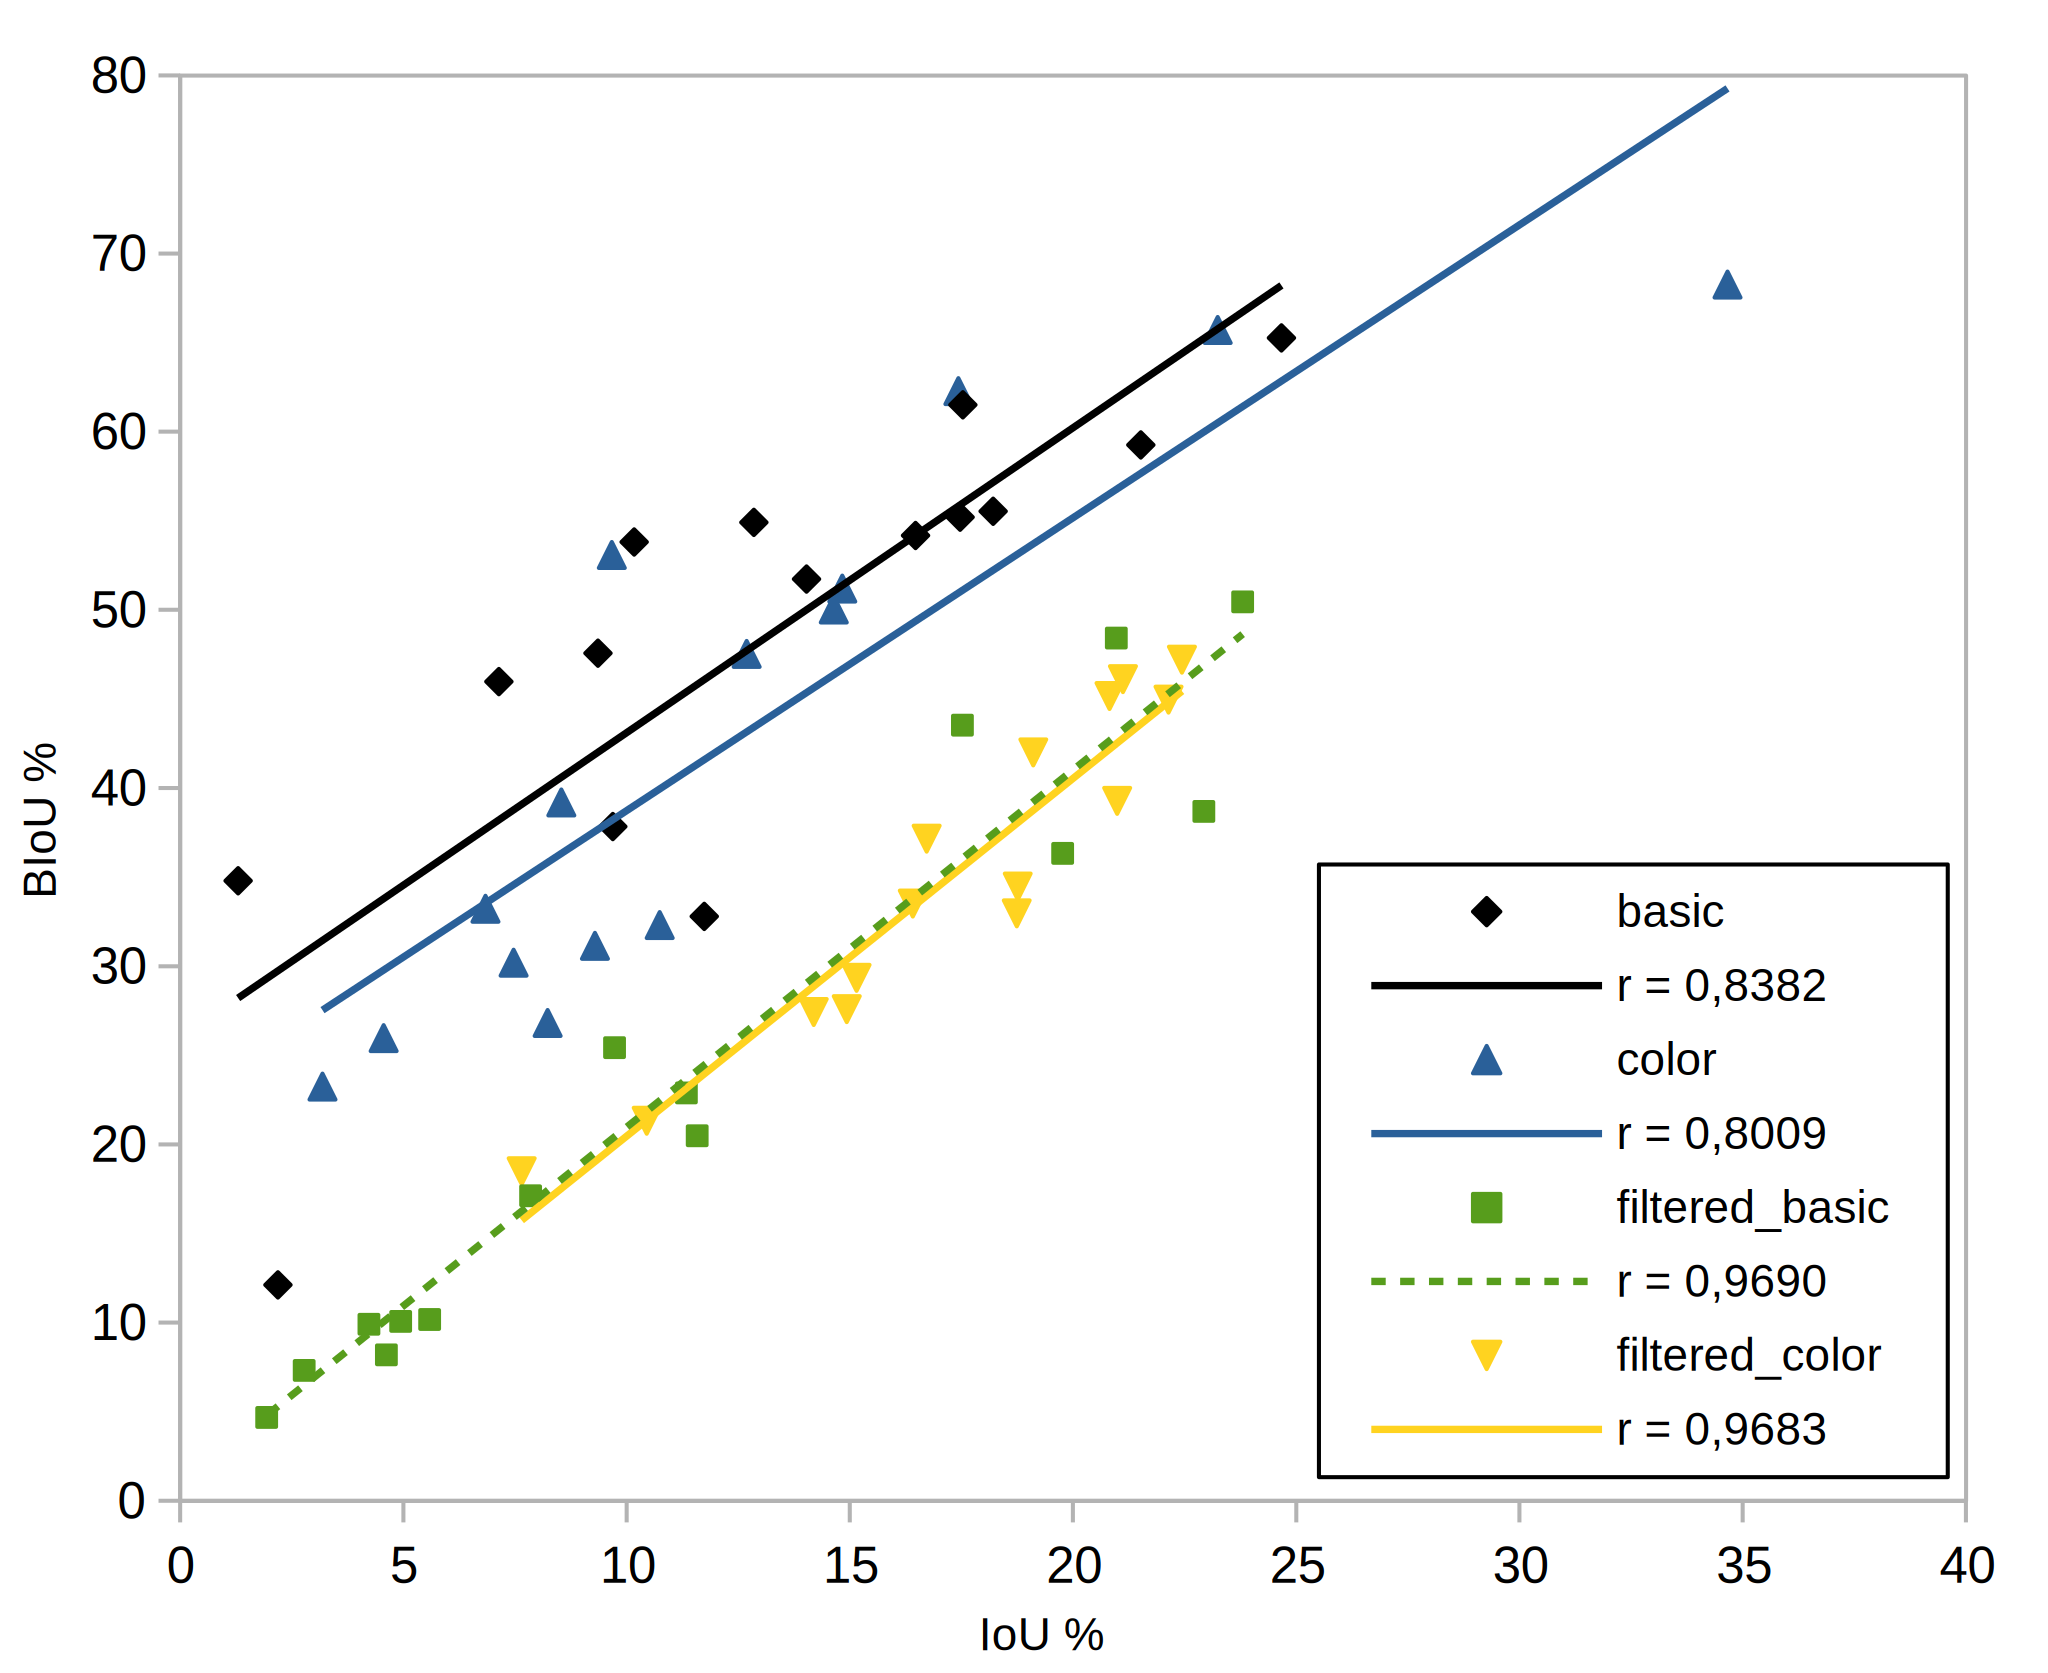
\includegraphics[width=0.65\textwidth]{Bilder/iou-biou-correlation-karlsruhe.pdf}
	\vspace{-5pt}
	% Das folgende ist ein Trick, um "Abbilgung x.y" in eine
	% eigene Zeile zu packen. Der Text zwischen [ und ] steht
	% im Abbildungsverzeichnis. Der Text darunter wird
	% tatsächlich angezeigt.
	\caption[BIoU der Modelle der Radwegerkennung auf dem Karlsruhe-Datensatz aufgetragen über deren IoU.]{\unskip}
	BIoU über IoU in Prozent für beide Augmentierungsmethoden und gefilterten und ungefilterten Karlsruhe-Datensatz 
	mit jeweils Korrelationskoeffizient. 
	\label{fig:iou-biou-corr-ka}
	% \vspace{-20pt}
\end{wrapfigure}

\autoref{fig:iou-biou-corr-ka} zeigt für den Karlsruhe-Datensatz in 
gefilterter und ungefilterter Variante und für beide Augmentierungsmethoden im Training für jedes Modell die BIoU aufgetragen 
über der IoU. Zusätzlich sind die ausschließlich positiven Korrelationskoeffizienten der jeweiligen Datenreihen angegeben. 
Zwischen IoU und BIoU des gefilterten Datensatzes herrscht eine sehr starke positive Korrelation ($r$ jeweils ~$0,96$), 
während der ungefilterte Datensatz eine schwächere positive Korrelation aufweist ($r_{basic} \approx 0,83$, 
$r_{color}\approx 0,8$). Das Diagramm veranschaulicht, dass, wie zuvor beschrieben, die BIoU auf 
dem gefilterten Datensatz signifikant niedriger ist als auf dem ungefilterten, während das für die IoU 
nicht zu beobachten ist. Auch ist die geringere Streuung auf den mit Color-Aug. trainierten Modellen auf dem 
gefilterten Karlsruhe-Datensatz durch die kürzere gelbe Strecke zu erkennen.  

\subsection{Ergebnisse bei fehlender Annotation}

Wie in \autoref{sec:bike-data} und \ref{sec:karlsruhe} beschrieben, wurde der BikeSat-Datensatz automatisch 
annotiert und der Karlsruhe-Datensatz von Menschen. Die Netze sind mit dem BikeSat-Datensatz trainiert. 
Wie bereits in \autoref{sec:bike-data} erwähnt, erhält die Datengrundlage zum BikeSat-Datensatz 
in einer von Menschen gesichteten und bewerteten Stichprobe \textbf{722} von \textbf{724} realen Radwegen.
Es fehlen also zwei Radwege. 

Die manuell von Menschen annotierten Bilder des Karlsruhe-Datensatzes zeigen dagegen eine höhere 
Fehlerquote. Die bestehenden Label sind zwar genauer platziert, aber dafür weniger vollständig. 
Hier ist bei einer Sichtung der Daten aufgefallen, dass ca. 15\% der Radwege nicht annotiert sind. 
Das hat aber keine Auswirkung auf das Training, da der Karlsruhe-Datensatz nur zum Testen verwendet wird.
\autoref{fig:annotation-mistake} zeigt ausgewählte Predictions (b)-(d) 
zu einem Ausschnitt aus dem Karlsruhe-Datensatz, bei dem bei der manuellen Annotation 
Radwege in der Straße, die von links unten nach rechts oben verläuft, übersehen wurden. 
In den Ausschnitten (c) und (d) sind die Radwege trotzdem erkannt, während es aber auch 
Beispiele wie (b) gibt, worin die querenden Radwege nicht getroffen sind. Ausschnitte (c) 
und (d) zeigen allerdings, dass die Netze Radwege erkennen können, die ein Mensch übersieht.
Es war allerdings kein Netz in der Lage für den gegebenen Bildausschnitt alle Radwege korrekt 
zu erkennen. \\
Was außerdem auffällig ist, ist, dass in Bild (c) der Radweg rechts unten genau getroffen ist 
(vgl. menschliche Annotation aus (a)), während in Bild (c) und (d) der Gehweg neben dem eigentlichen 
Radweg annotiert ist. Zudem fällt in (d) ein grober Fehler des Netzes auf, da hier klar Teile des 
blauen Dachs auf der rechten Bildseite annotiert sind.

\begin{figure}
	\centering
	\begin{subfigure}{.45\textwidth}
		\centering
		\includegraphics[width=1.\linewidth]{Bilder/annotation-mistake/overlayed.png}
		\caption{}
	\end{subfigure}
	\begin{subfigure}{.45\textwidth}
		\centering
		\includegraphics[width=1.\linewidth]{Bilder/annotation-mistake/straight-dbunet-r.png}
		\caption{}
	\end{subfigure} 
	\begin{subfigure}{.45\textwidth}
		\centering
		\includegraphics[width=1.\linewidth]{Bilder/annotation-mistake/fitting-vbunet-r.png}
		\caption{}
	\end{subfigure}
	\begin{subfigure}{.45\textwidth}
		\centering
		\includegraphics[width=1.\linewidth]{Bilder/annotation-mistake/full-vbunet-s.png}
		\caption{}
	\end{subfigure}

	\caption{(a) zeigt ein manuell annotierten Ausschnitt aus dem Karlsruhe-Datensatz, wobei Radwege 
	fälschlicherweise nicht annotiert sind. Abbildungen (b), (c) und (d) zeigen die Predictions von \ac{DBUNet}$^r$,
	\ac{VBUNet}$^r$, bzw. \ac{VBUNet}$^*$.}
	\label{fig:annotation-mistake}
\end{figure}

% networks tested with karlsruhe test data set  

% testing ./../Models/Double-Data\backbones\bike_mapper_pre-train-scratch-densenet121_Aug_IoU3076_q6178.h5
% iou: 0.07135618478059769, quality:0.45967867970466614

% testing ./../Models/Double-Data\backbones\bike_mapper_pre-train-scratch-resnet34_Aug_IoU2911_q6053.h5
% iou: 0.11737822741270065, quality:0.3280484974384308

% testing ./../Models/Double-Data\backbones\bike_mapper_pre-train-scratch-vgg16_Aug_IoU3045_q6148.h5
% iou: 0.09694375097751617, quality:0.3783626854419708

% testing ./../Models/Double-Data\pre-train\bike_mapper_pre-train-freeze-left_Aug_IoU2448_q5177.h5
% iou: 0.020918812602758408, quality:0.1211065948009491

% testing ./../Models/Double-Data\pre-train\bike_mapper_pre-train-freeze-right_Aug_IoU2535_q5127.h5
% iou: 0.09364935010671616, quality:0.47571051120758057

% testing ./../Models/Double-Data\pre-train\bike_mapper_triple-param_pre-train-freeze-left_Aug_IoU2814_q5714.h5
% iou: 0.1647404581308365, quality:0.5417148470878601

% testing ./../Models/Double-Data\pre-train\bike_mapper_triple-param_pre-train-freeze-right_Aug_IoU2822_q5726.h5
% iou: 0.10167630761861801, quality:0.5381019115447998

% testing ./../Models/Double-Data\road-pre-trained-backbones\bike_mapper_pre-train-densenet121freeze-left_Aug_IoU3155_q6238.h5
% iou: 0.17469285428524017, quality:0.5520145893096924

% testing ./../Models/Double-Data\road-pre-trained-backbones\bike_mapper_pre-train-densenet121freeze-right_Aug_IoU3212_q6299.h5
% iou: 0.14031212031841278, quality:0.5172706246376038

% testing ./../Models/Double-Data\road-pre-trained-backbones\bike_mapper_pre-train-resnet34freeze-left_Aug_IoU3098_q6051.h5
% iou: 0.24674279987812042, quality:0.6527144312858582

% testing ./../Models/Double-Data\road-pre-trained-backbones\bike_mapper_pre-train-resnet34freeze-right_Aug_IoU3131_q6355.h5
% iou: 0.18207795917987823, quality:0.5552724599838257

% testing ./../Models/Double-Data\road-pre-trained-backbones\bike_mapper_pre-train-vgg16freeze-left_Aug_IoU3224_q6293.h5
% iou: 0.12852726876735687, quality:0.5490880012512207

% testing ./../Models/Double-Data\road-pre-trained-backbones\bike_mapper_pre-train-vgg16freeze-right_Aug_IoU3184_q6151.h5
% iou: 0.175296351313591, quality:0.6151095628738403

% testing ./../Models/Double-Data\bike_mapper_scratch_Aug_IoU2354_q4771.h5
% iou: 0.013092363253235817, quality:0.3479517698287964

% testing ./../Models/Double-Data\bike_mapper_scratch_triple-param_Aug_IoU2793_q5655.h5
% iou: 0.21523651480674744, quality:0.5924956798553467

